\documentclass[./../../paper.tex]{subfiles}
\graphicspath{{\subfix{./../../figures/}}}

\begin{document}

In order to explain the decisions of a prediction we have to introduce a predictive model, which needs to be explained. Any sequence model suffices. Additionally, the model's prediction do not have to be accurate. However, the more accurate the model can capture the dynamics of the process, the better the counterfactual functions as an explanation of these dynamics. This becomes particularly important if the counterfactuals are assessed by a domain expert. 

\subsection{Long Short-Term Memory Models}
\label{sec:lstm_prediction_model}
In this thesis, the predictive model is an \gls{LSTM} model. LSTMs are well-known models within \gls{DL}, that use their structure to process sequences of variable lengths\autocite{hochreiter_LongShortTermMemory_1997}. LSTMs are an extension of \glspl{RNN}. We choose this model as it is simple to implement and can handle long-term dependencies well.

Generally, \glspl{RNN} are \glspl{NN} that maintain a state $h_{t+1}$. The state ist computed and then propagated to act as an additional input alongside the next sequential input of the instance $x_{t+1}$. The hidden state $h$ is also used to compute the prediction $o_{t}$ for the current step. The formulas attached to this model are shown in 

\begin{align}
    \label{eq:rnn}
    h_{t+1} &= \sigma(V h_t + U x_t + b)\\
    o_{t} &= \sigma(W h_t + b)
\end{align}

Here, $W$, $U$ and $V$ are weight matrices that are multiplied with their respective input vectors $h_t$, $x_t$. $b$ is a bias vector and $\sigma$ is a nonlinearity function. LSTM fundamentally work similarly, but have a more complex structure that allows to handle long-term dependencies better. They manage this behaviour by introducing addional state vectors, that are also propagated to the following step. We omit discussing these specifics in detail, as their explanation is not further relevant for this thesis. For our understanding it is enough to know that $h_t$ holds all the necessary state information. \autoref{fig:rnn} shows a schematic representation of an RNN.   

\begin{figure}[htb]
    \label{fig:rnn}
    \centering
    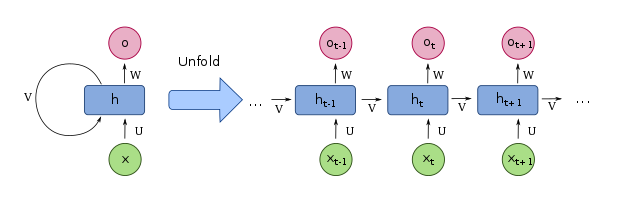
\includegraphics[width=0.9\textwidth]{figures/rnn.png}
    \caption{A schematic representation of an RNN viewed in compact and unfolded form\autoref{_RecurrentNeuralNetwork_2022a}.}
\end{figure}

\subsubsection{Model Architecture}

\subsection{Transformer Model}
Transformer model are modern sequnetial models within \gls{DL}. They have a multitude of advantages over sequential models such as \glspl{RNN} or \glspl{LSTM}\autocite{vaswani_AttentionAllYou_2017}. First, they do not need to be computed sequentially. Hence, it is possible to parallelise the training and inference substantially using GPUs. Second, they can take the full sequence as an input using the attention mechanism. This mechanism also allows to inspect which inputs have had a significant role into producing the prediction. However, transformer models are more complicated to implement. The overall setup is shown in \autoref{fig:transformer}\autocite{vaswani_AttentionAllYou_2017}.

\begin{figure}[htb]
    \centering
    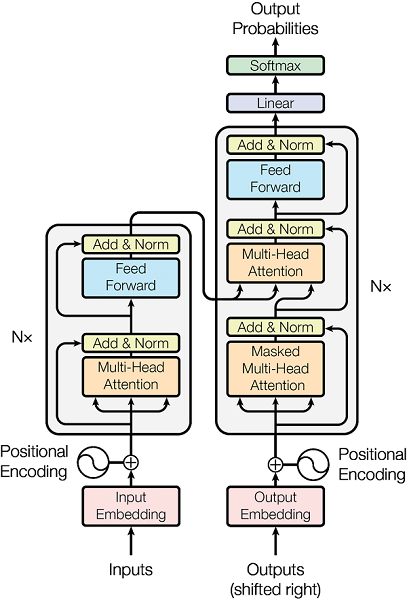
\includegraphics[width=0.5\textwidth]{figures/transformer.png}
    \caption{A schematic representation of a Transformer model.}
    \label{fig:transformer}
\end{figure}

The transformer model is an Encoder-Decoder model. The encoder takes in the input sequence as a whole and generates a vector which encodes the information. The decoder uses the econding to produce the resulting sequence. The encoder module uses two important concepts. First, in order to preserve the temporal information of the input we encode the position of each sequential input as an additional input vector. We choose to encode every position by jointly learning  positional embeddings. The second component is multihead-self-attention. According to \citeauthor{vaswani_AttentionAllYou_2017}, we can describe attention as a function which maps a query and a set of key-value pairs to an output. More specifically, self attention allows us to relate every input element in the sequence to be related to any other sequence in the input. The output is a weighted sum of the values. It is possible to stack multiple self-attention modules. This procedure is called multihead-attention. \autoref{fig:selfattention} shows how to compute self-attention accoring to \autoref{eq:selfattention}\autocite{vaswani_AttentionAllYou_2017}. 


\begin{figure}[htb]
    \centering
    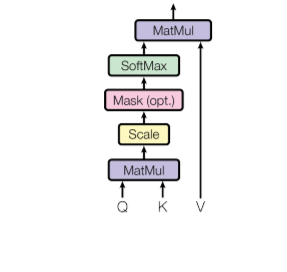
\includegraphics[width=0.5\textwidth]{figures/selfattention.png}
    \caption{Shows the computational graph of self-attention. $Q, K \text{ and } V$ are all the same input sequence. $Q$ stands for query, $K$ for key and $V$ for value.}
    \label{fig:selfattention}
\end{figure}


\begin{align}
    \label{eq:selfattention}
    Attention(Q, K, V) &= softmax(\frac{QK^T}{\sqrt{d_k}})V 
\end{align}

$Q, K, V$ are all the same input sequence. $d_k$ refers to the dimension of an input vector. Note, that $T$ is the transpose operation of matrix computations and does not relate to the time step of the final sequence element. 

\subsubsection{Model Architecture}

\end{document}